\documentclass[10pt,a4paper]{article}
% Submission-audit note: bibliography and related-work search refreshed on 2026-10-04; author information updated for submission.

\usepackage[margin=0.78in]{geometry}
\usepackage{amsmath,amssymb,mathtools}
\usepackage{amsthm}
\usepackage{booktabs}
\usepackage{array}
\usepackage{tabularx}
\usepackage{multirow}
\usepackage{enumitem}
\usepackage{microtype}
\usepackage{graphicx}
\usepackage{tikz}
\usetikzlibrary{arrows.meta,positioning,calc,fit,decorations.pathreplacing}
\usepackage{xcolor}
\usepackage[hidelinks]{hyperref}
\usepackage{url}
\usepackage{caption}
\usepackage{subcaption}
\usepackage{fancyvrb}
\usepackage{float}
\usepackage{placeins}

\setlength{\parindent}{0pt}
\setlength{\parskip}{0.45em}
\setlist[itemize]{leftmargin=1.5em,itemsep=0.18em,topsep=0.25em}
\setlist[enumerate]{leftmargin=1.7em,itemsep=0.18em,topsep=0.25em}
\renewcommand{\arraystretch}{1.12}
\newcolumntype{L}[1]{>{\raggedright\arraybackslash}p{#1}}
\captionsetup{font=small,labelfont=bf,justification=justified,singlelinecheck=false}
\setlength{\textfloatsep}{10pt plus 2pt minus 2pt}
\setlength{\floatsep}{9pt plus 2pt minus 2pt}
\setlength{\intextsep}{9pt plus 2pt minus 2pt}

\newcommand{\F}{\mathbb{F}}
\newcommand{\HW}{\operatorname{HW}}
\newcommand{\E}{\mathbb{E}}
\newcommand{\Prb}{\Pr}
\providecommand{\ket}[1]{\lvert #1\rangle}
\newcommand{\WARP}{\textsc{WARP}}
\newcommand{\Sb}{S_{b0}}
\newtheorem{proposition}{Proposition}
\newtheorem{corollary}[proposition]{Corollary}
\newtheorem{remark}[proposition]{Remark}

\title{\textbf{Quantum Key Search on WARP-128:}\\
Verified Reversible Circuits, Multi-Pair Identifiability,\\
and Success-Normalized Grover Analysis}

\author{
Indranil Mukherjee\\
\small Indian Institute of Technology Jodhpur, Jodhpur, Rajasthan, India\\
\small \texttt{p25ma0005@iitj.ac.in}
\and
Bimal Mandal\\
\small Indian Institute of Technology Jodhpur, Jodhpur, Rajasthan, India\\
\small \texttt{bimalmandal@iitj.ac.in}
}
\date{}

\begin{document}
\maketitle

\begin{abstract}
We present a verified quantum key-search analysis of the complete 41-round lightweight block cipher WARP-128. The baseline reversible encryption uses 256 logical qubits, 2,763 X gates, 10,496 CNOTs, and 5,248 Toffoli gates. We construct several two-pair Grover oracles and quantify their width--gate--depth tradeoffs: a gate-oriented iteration uses 21,750 Toffolis, while balanced equality and coherent key fanout reduce the complete-iteration Toffoli-layer depth from 1,156 to 358 at increased width. Under the ideal-permutation model we derive the exact known-plaintext identifiability law; for WARP's equal 128-bit key and block sizes, one pair uniquely determines the generating key with probability approaching $e^{-1}$, whereas two pairs leave only $2^{-128}$ expected wrong survivors. We apply fixed-confidence restart accounting so that reduced per-run Grover depth is not conflated with aggregate recovery work, and show how noise can shift the preferred stopping point. As a cross-cipher extension, exhaustive Mini-AES and S-AES experiments validate the one-pair/multi-pair distinction in small domains. Full-round sparse experiments and a separate Toy-WARP-8 Qiskit/Aer demonstrator provide executable checks without claiming near-term full-scale recovery.
\end{abstract}

\section{Introduction}

Grover's search algorithm gives a generic quadratic speedup for exhaustive search over an unstructured key space~\cite{Grover1996}. For a block cipher with a $k$-bit key, the query complexity of generic quantum exhaustive search is therefore on the order of $2^{k/2}$, but the practical logical cost depends critically on how the encryption function and the key-checking predicate are realized as reversible quantum circuits. This has motivated detailed circuit-level studies for AES and Rijndael~\cite{Grassl2016,Langenberg2020,Jaques2020,Lin2023,SongSeo2026}, lightweight block ciphers such as PRESENT, GIFT, DEFAULT, PRINCE, Midori, KLEIN, SLIM, and MIBS~\cite{Jang2021,JangDefault2025,Akhlaq2024,KLEIN2026,SLIM2025,MIBS2026}, and executable small-cipher demonstrations~\cite{Wang2025,Kiran2026}.

WARP~\cite{WARP2020} is a lightweight 128-bit block cipher with a 128-bit key. Its state consists of 32 nibbles and its round function is a Type-2 generalized Feistel network (GFN) using the MIDORI $4$-bit S-box, a simple alternating-half key schedule, round constants, and a fixed nibble permutation. The cipher was designed for compact hardware implementations while retaining a full 128-bit block size. The generalized-Feistel structure is also attractive from the viewpoint of reversible computing because one branch can be updated while the companion branch is preserved.

Quantum analysis of generalized Feistel structures has been studied in chosen-query and related-key settings, including Simon-based distinguishers and key-recovery techniques for several GFN families~\cite{Dong2019,Hodzic2022,Sun2023,Sun2026}. The 2026 work of Sun et al.~\cite{Sun2026} is especially relevant structurally because it gives polynomial-query secret-state recovery for generic Type-1/2 generalized Feistel schemes under quantum related-key access and independent-subkey assumptions. Those assumptions differ materially from the known-plaintext Grover model and the alternating-half WARP master-key schedule considered here, so the result is complementary rather than a direct replacement for a concrete WARP oracle implementation.

The quantum-circuit literature has also expanded to Feistel and generalized-Feistel lightweight designs. Rahman and Paul~\cite{Rahman2022} give depth-aware Grover resource estimates for KATAN, while recent studies of SLIM and MIBS use multi-pair Grover checking under NIST-style depth constraints~\cite{SLIM2025,MIBS2026}. Ulgen et al.~\cite{Ulgen2026} construct a full quantum circuit and parallel multi-pair Grover oracle for the hybrid generalized-Feistel cipher GFSPX. To the best of our knowledge, after a targeted literature search updated through 5 October 2026, we did not identify prior work giving a complete reversible implementation together with a known-plaintext Grover-oracle resource analysis specifically for WARP-128. The novelty claim is therefore deliberately limited to this WARP-specific implementation, oracle, verification, and resource-analysis scope.

The recent Mini-AES study of Kiran et al.~\cite{Kiran2026} and the S-AES study of Wang et al.~\cite{Wang2025} show the value of small ciphers as executable laboratories for Grover key search, circuit optimization, and noise analysis.  They also expose a methodological distinction that becomes essential for a full-size cipher: a shallow Grover run, a detectable marked state, and a low-cost unique-master-key recovery are different claims.  We therefore separate (i) the number of keys satisfying the supplied known pairs, (ii) per-run amplitude-amplification success, and (iii) aggregate work required to reach a fixed overall recovery probability.  WARP is a particularly clean full-size case because its key and block sizes are equal, so a single known pair is not expected to define a unique-key predicate even for an ideal cipher.

\paragraph{Contributions.}
Our main contributions are as follows.
\begin{itemize}
    \item We give a verified reversible implementation of the complete 41-round WARP-128 encryption function. The implementation uses 128 state qubits and 128 quantum key qubits, requires no additional clean ancilla in the baseline encryption, and is checked against all three official test vectors and 100 random full-encryption comparisons.
    \item We independently synthesize and exhaustively verify a 10-gate in-place realization of the WARP/MIDORI $S_{b0}$ S-box in the NCT library. We then construct the actual WARP Feistel nonlinear primitive $\ket{x}\ket{y}\mapsto\ket{x}\ket{y\oplus S(x)}$ using compute--copy--uncompute with no ancilla.
    \item We construct a one-pair Grover phase oracle and three collision-aware two-pair architectures, exposing a clear qubit--gate tradeoff. The gate-oriented two-pair construction uses 637 qubits, while a compact recomputation construction reduces this to 383 qubits at higher gate and depth cost.
    \item We derive an exact known-plaintext identifiability law under the ideal-permutation model.  For $r$ distinct pairs, the number of wrong keys satisfying all pairs is binomial with mean $(2^k-1)/(2^b)_r$.  For WARP ($k=b=128$), one pair uniquely identifies the true key with probability approximately $e^{-1}$, while two pairs reduce the expected number of wrong survivors exactly to $2^{-128}$.
    \item We validate the identifiability interpretation independently on Mini-AES and S-AES by exhaustive enumeration of all $2^{16}$ keys.  In both ciphers a tested single pair admits three satisfying keys, while a second pair reduces the common satisfying set to the intended master key.  A pre-declared 16-plaintext occupancy experiment gives no multiple-testing-corrected evidence that this one-pair multiplicity is exceptional relative to a random key-to-ciphertext mapping baseline.
    \item We provide executable key-recovery experiments that retain the full 41-round WARP encryption function and restrict only a subset of master-key bits to be unknown. The marked set is validated using the actual reversible NCT gate list, and the resulting Grover amplitudes agree with the exact closed-form formula to machine precision.
    \item We complement the full-WARP experiment with an explicitly reduced 8-bit WARP-structured demonstrator for complete end-to-end execution. The reversible Toy-WARP-8 circuit is exhaustively checked on all $2^{16}=65{,}536$ key/plaintext inputs; a real Qiskit/Aer Grover run over all 256 keys recovers $K=\mathtt{C6}$ in 4,095 of 4,096 shots after 12 iterations. A controlled three-seed depolarizing campaign then quantifies the tradeoff between amplitude amplification, accumulated circuit noise, and fixed-success repetition cost.
    \item We apply success-normalized Grover accounting systematically: a reduced per-run iteration count is compared only after including the independent-restart factor required to reach a common overall success probability.  We combine this with exact finite-shot binomial calculations and explicitly parameterized stochastic-Pauli noise experiments, showing how noise can shift the fixed-confidence optimum toward earlier stopping.  These simulations are not interpreted as evidence that the full WARP oracle is executable on present NISQ hardware.
    \item We add a depth-oriented oracle family based on balanced AND trees and coherent computational-basis key fanout. The best depth-oriented construction keeps essentially the same Toffoli and $T$ counts as the gate-oriented oracle but reduces the Toffoli-layer depth of a complete two-pair Grover iteration from 1,156 to 358, exposing an explicit width--$T$-depth tradeoff.
    \item We formalize the exact sparse-simulation principle underlying the executable experiments. Because the reversible WARP circuit is a computational-basis permutation and the key register is retained, a superposition over $2^u$ candidate keys remains supported on exactly $2^u$ basis branches throughout encryption; no dense $2^{256}$ statevector is required.
\end{itemize}

\section{Related Work}
Grassl et al.~\cite{Grassl2016} established detailed reversible resource estimates for Grover key search on AES, including qubits, depth, and logical gate counts. Subsequent work refined AES circuit costs and oracle engineering~\cite{Langenberg2020,Jaques2020,Lin2023}. Song and Seo~\cite{SongSeo2026} recently extended verified quantum-resource estimation to the Rijndael family under the NIST MAXDEPTH model, reinforcing the importance of reporting both width and depth rather than a single gate count.

Lightweight ciphers have received similarly broad attention. Jang et al.~\cite{Jang2021} implemented PRESENT and GIFT, and their later DEFAULT study compares alternative reversible design choices under Grover search~\cite{JangDefault2025}. Jing et al.~\cite{Jing2023} analyzed LBlock and LiCi, while Akhlaq et al.~\cite{Akhlaq2024} reported quantum resources for PRINCE and Midori. More recent studies cover the KLEIN family~\cite{KLEIN2026}, the Feistel ciphers SLIM and MIBS~\cite{SLIM2025,MIBS2026}, and the hybrid GFN/ARX-SPN design GFSPX~\cite{Ulgen2026}. These papers use different gate libraries, parallelization assumptions, and security metrics, so numerical resource totals should be compared only within explicitly stated cost models.
Because dense statevector simulation of a realistic full block-cipher oracle is classically prohibitive, several works use simplified or reduced ciphers to demonstrate end-to-end Grover behavior. Moiseevskiy~\cite{Moiseevskiy2023} studied S-AES with reduced qubit counts under partial-key leakage. Wang et al.~\cite{Wang2025} subsequently developed a resource-reduced S-AES attack, while Kiran et al.~\cite{Kiran2026} implemented Mini-AES, performed known-plaintext Grover recovery, analyzed module noise, and used finite-shot arguments to motivate reduced iteration counts.  These studies provide useful executable baselines, but their small equal-size key/block domains also make visible a generic issue that is easy to overlook: a single plaintext/ciphertext pair need not identify a unique key.  We use Mini-AES and S-AES later only as exhaustive small-domain validation targets for this identifiability question; the cryptographic target of the present work remains full 41-round WARP-128.

Our executable experiments take a different reduction strategy. We do not define a new reduced-round or reduced-state version of WARP. Instead, we retain the full 41-round encryption function and restrict only the number $u$ of unknown master-key bits. This preserves the exact WARP round structure and allows direct regression against the independent classical implementation.
WARP has received substantial classical analysis, and this context is important when interpreting a quantum exhaustive-search baseline. Teh and Biryukov~\cite{Teh2022} gave differential and related-key cryptanalysis, including a 23-round key-recovery attack from an 18-round differential distinguisher. Hadipour and Eichlseder~\cite{Hadipour2022} developed a bit-oriented monomial-prediction model and extended integral key recovery to 32 of the 41 rounds, with the final complexity dominated by $2^{127}$ chosen plaintexts. Shi et al.~\cite{Shi2023} independently evaluated WARP against linear cryptanalysis using SAT-based trail and hull search and extended the linear analysis beyond the designers' original bounds. Zeng, Tan, and Xu~\cite{Zeng2025} subsequently improved boomerang distinguishers and obtained a 27-round rectangle attack. A 2026 automated low-data meet-in-the-middle framework also reports an 18-round known-plaintext attack on WARP using seven known plaintexts~\cite{Vaziri2026}. None of these results constitutes a full-round practical break, but they identify reduced-round structure that could support future dedicated quantum cryptanalysis beyond generic Grover search.
The 4-bit nonlinear layer is often the dominant design problem in lightweight reversible circuits. LIGHTER-R~\cite{Dasu2019} searches for low-cost reversible implementations of 4-bit S-boxes, while DORCIS~\cite{DORCIS2023} extends this line toward quantum- and $T$-depth-oriented synthesis. Chen et al.~\cite{Chen2024} formulate a SAT-based quantum-circuit decision problem and report depth-oriented realizations for several S-boxes, including MIDORI. These works provide appropriate external reference points for the same S-box used by WARP. In our implementation we independently recover the 10-gate NCT realization and verify it exhaustively; we do not claim a new S-box depth record.
Quantum distinguishers and key-recovery attacks on Feistel and generalized Feistel constructions have been studied using Simon-type periodicity and related methods~\cite{Dong2019,Hodzic2022,Sun2023,Sun2026}. In particular, Sun et al.~\cite{Sun2026} show that generic Type-1/2 GFS structures can admit polynomial-query secret-state recovery in a quantum related-key model when independent-subkey and oracle assumptions hold. This makes it important to distinguish the attack model from ordinary known-plaintext Grover search: the present work assumes classical known plaintext/ciphertext pairs and a quantum circuit evaluating WARP under candidate master keys, not a superposition-access related-key oracle. Liu and Yang~\cite{LiuYang2020} additionally demonstrate how a classical differential property can be combined with quantum search to outperform generic exhaustive search on reduced-round SIMON. These results motivate a separate future question for WARP: whether its published reduced-round differential or integral key-recovery structure can be translated into a dedicated quantum attack with a lower cost than the full-key Grover baseline.

\section{Preliminaries}

\subsection{Grover search}
Let a search space contain $N$ candidates, of which $M$ are marked. Define
\begin{equation}
    \sin^2\theta = \frac{M}{N}, \qquad 0<\theta\le \frac{\pi}{2}.
\end{equation}
After $j$ Grover iterations, the total marked-state success probability is
\begin{equation}
    P_j = \sin^2\bigl((2j+1)\theta\bigr).
    \label{eq:grover_success}
\end{equation}
For $M\ll N$, the first maximum occurs near
\begin{equation}
    j^* \approx \frac{\pi}{4}\sqrt{\frac{N}{M}}.
    \label{eq:grover_iterations}
\end{equation}
A complete Grover iteration contains a phase oracle and a diffuser. Consequently, a realistic cost estimate must multiply the iteration count by the cost of both operations.

\subsection{Fixed-confidence restart normalization}
\label{subsec:fixed_confidence}
A smaller number of Grover iterations in one execution does not by itself imply a cheaper key-recovery attack.  If a run stopped after $j$ iterations succeeds with probability $p_j$ and the desired overall success probability is $\eta$, then $R$ independent runs fail jointly with probability $(1-p_j)^R$.  Hence the minimum repetition count is
\begin{equation}
    R_{\eta}(j)=
    \left\lceil
    \frac{\log(1-\eta)}{\log(1-p_j)}
    \right\rceil .
    \label{eq:restart_factor}
\end{equation}
For the boundary cases we take $R_{\eta}(j)=1$ when $p_j=1$ and no finite repetition count when $p_j=0$ (for $0<\eta<1$). For $0<p_j<1$, Eq.~\eqref{eq:restart_factor} is well defined.

The serial query-equivalent cost is therefore
\begin{equation}
    Q_{\eta}(j)=jR_{\eta}(j).
    \label{eq:fixed_success_cost}
\end{equation}
More generally, if a resource has per-run fixed overhead $G_0$ and per-iteration cost $G_{\rm iter}$, its success-normalized aggregate cost is
\begin{equation}
    G_{\eta}(j)=R_{\eta}(j)\bigl(G_0+jG_{\rm iter}\bigr).
    \label{eq:fixed_success_resource}
\end{equation}
This normalization can be applied to logical gate count, $T$ count, or other additive resources.  If the repetitions are executed serially, $Q_{\eta}(j)$ measures aggregate iteration work.  If they are executed concurrently on independent processors, wall-clock depth can be reduced only by paying a corresponding width/hardware factor.  We therefore keep per-run depth, aggregate fixed-confidence work, and parallel hardware cost conceptually separate.

\subsection{Resource metrics}
We report logical qubit count, X, H, CNOT, CZ, Toffoli (CCX), total gate count, and a transparent weighted NCT depth in which
\begin{equation}
    w(X)=w(\mathrm{CNOT})=1,\qquad w(\mathrm{CCX})=7.
\end{equation}
This weighted depth is an internal logical metric and is not the same as fault-tolerant $T$-depth.

For Clifford+$T$ accounting we use two exact-Toffoli models. In model FT-A, each Toffoli uses seven $T$ gates, $T$-depth three, and no decomposition ancilla, following the depth-three exact realization of Amy et al.~\cite{Amy2013}. In model FT-B, the same seven-$T$ Toffoli is assigned $T$-depth one using four clean ancillas as in Selinger~\cite{Selinger2013}. The latter is a deliberately width-intensive depth model. We compute the circuit's \emph{Toffoli-layer depth} with a dependency-aware ASAP pass: Clifford gates add no $T$ layer but propagate dependencies between all wires they touch, while a CCX increments the maximum incoming layer. Thus
\begin{equation}
T\text{-depth}_{\rm FT-A}=3D_{\rm CCX},\qquad
T\text{-depth}_{\rm FT-B}=D_{\rm CCX}.
\end{equation}
For FT-B we additionally report the conservative width upper bound obtained by assigning four decomposition ancillas to every simultaneously scheduled CCX. These models are logical fault-tolerant accounting conventions; surface-code routing, distillation, and architecture-specific timing remain outside scope.

\section{The WARP-128 Block Cipher}

WARP~\cite{WARP2020} has a 128-bit block and a 128-bit master key. The state is written as
\begin{equation}
    X = X_0\|X_1\|\cdots\|X_{31}, \qquad X_i\in\F_2^4.
\end{equation}
The key is split into two 64-bit halves,
\begin{equation}
    K = K^{(0)}\|K^{(1)},
\end{equation}
with each half represented by 16 nibbles. The halves are used alternately across rounds, starting with $K^{(0)}$.

For $i=0,\ldots,15$, the nonlinear/key update in zero-based round $r$ is
\begin{equation}
    X_{2i+1}\leftarrow X_{2i+1}\oplus \Sb(X_{2i})\oplus K^{(r\bmod 2)}_i.
    \label{eq:warp_subround}
\end{equation}
Two round-constant nibbles are then XORed into fixed state positions. Rounds 1--40 apply the WARP nibble permutation, while the final round omits the permutation.

\begin{table}[t]
\centering
\caption{The WARP/MIDORI $S_{b0}$ S-box.}
\label{tab:sbox}
\begin{tabular}{c|*{16}{c}}
\toprule
$x$ & 0 & 1 & 2 & 3 & 4 & 5 & 6 & 7 & 8 & 9 & A & B & C & D & E & F\\
\midrule
$S(x)$ & C & A & D & 3 & E & B & F & 7 & 8 & 9 & 1 & 5 & 0 & 2 & 4 & 6\\
\bottomrule
\end{tabular}
\end{table}

The nibble permutation used in our implementation is
\begin{align}
\pi = [&31,6,29,14,1,12,21,8,27,2,3,0,25,4,23,10,\nonumber\\
       &15,22,13,30,17,28,5,24,11,18,19,16,9,20,7,26].
\end{align}
It decomposes into two 16-cycles. In the logical circuit we therefore treat the permutation as a relabeling of wires rather than as a sequence of physical SWAP gates. Hardware-specific routing is discussed separately in Section~\ref{sec:limitations}.

\begin{figure}[tbp]
\centering
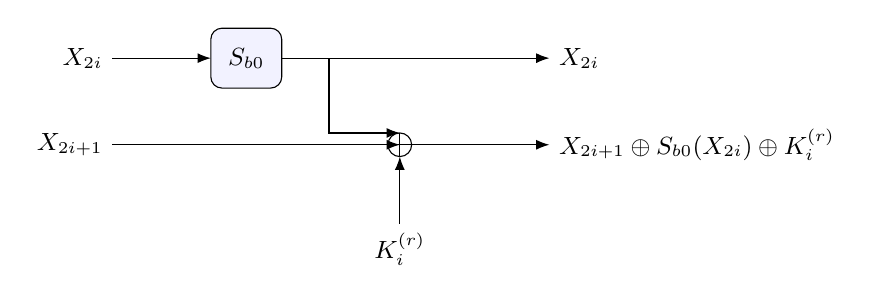
\begin{tikzpicture}[>=Latex,x=1cm,y=1cm,every node/.style={font=\small}]
% Even branch
\draw[->] (0,1.1) -- (1.25,1.1);
\node[left] at (0,1.1) {$X_{2i}$};
\draw[fill=blue!5,rounded corners] (1.25,0.72) rectangle (2.15,1.48);
\node at (1.70,1.10) {$\Sb$};
\draw[->] (2.15,1.1) -- (5.55,1.1);
\node[right] at (5.55,1.1) {$X_{2i}$};
% Odd branch
\draw[->] (0,0) -- (3.65,0);
\node[left] at (0,0) {$X_{2i+1}$};
\draw (3.65,0) circle (0.15);
\draw (3.50,0)--(3.80,0);
\draw (3.65,-0.15)--(3.65,0.15);
\draw[->] (3.80,0) -- (5.55,0);
\node[right] at (5.55,0) {$X_{2i+1}\oplus \Sb(X_{2i})\oplus K_i^{(r)}$};
% S output into XOR
\draw[->] (2.75,1.1) |- (3.65,0.15);
% key input
\draw[->] (3.65,-1.0) -- (3.65,-0.15);
\node[below] at (3.65,-1.0) {$K_i^{(r)}$};
\end{tikzpicture}
\caption{One WARP Feistel subround. The even nibble is preserved, while its S-box output and the active round-key nibble are XORed into the odd nibble. Sixteen such branches are evaluated in parallel in each round.}
\label{fig:warp_subround}
\end{figure}

\section{Reversible Quantum Implementation of WARP}

\subsection{S-box synthesis}
Using the bit convention $x=x_0+2x_1+4x_2+8x_3$, we independently synthesized a 10-gate in-place NCT circuit for Table~\ref{tab:sbox}. The circuit contains
\begin{equation}
    2\,X + 4\,\mathrm{CNOT} + 4\,\mathrm{CCX},
\end{equation}
with a free output-wire relabeling
\begin{equation}
    y_0\leftarrow q_1,\quad y_1\leftarrow q_2,\quad y_2\leftarrow q_3,\quad y_3\leftarrow q_0.
\end{equation}
The circuit in Figure~\ref{fig:sbox_block_circuit} was exhaustively checked on all 16 inputs. A meet-in-the-middle search over the complete four-qubit NCT library, allowing all 24 output permutations, found no solution below 10 gates and found a solution at 10 gates. Thus the gate count is optimal for the declared four-qubit NCT gate library with free output-wire permutation. The submission audit includes an independent bidirectional-search certificate for this statement. The resulting weighted full depth is 32. For comparison, Chen et al.~\cite{Chen2024} report a depth-31 MIDORI realization under their SAT model; our result therefore serves as an independently verified compact implementation rather than a new depth record.

\begin{figure}[tbp]
\centering
\resizebox{0.95\textwidth}{!}{%
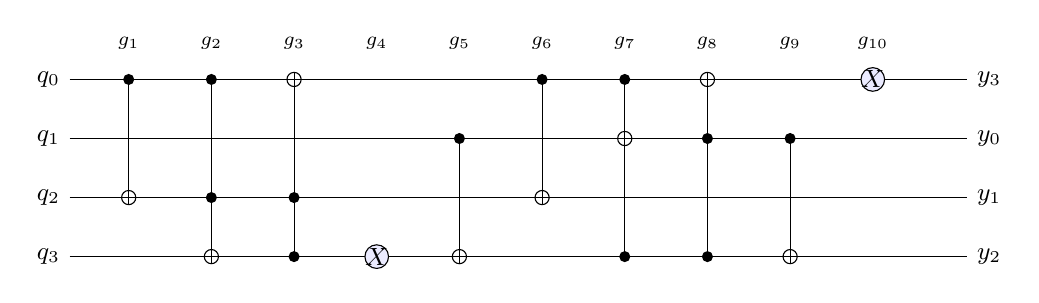
\begin{tikzpicture}[x=0.75cm,y=0.75cm,>=Latex,every node/.style={font=\small}]
% four wires
\foreach \r/\lab in {0/{q_0},1/{q_1},2/{q_2},3/{q_3}}{
  \draw (0,-\r) -- (15.2,-\r);
  \node[left] at (0,-\r) {$\lab$};
}
% helper-like gates drawn explicitly
% G1 CX q0->q2
\fill (1.0,0) circle (2pt); \draw (1.0,0)--(1.0,-2); \draw (1.0,-2) circle (0.12); \draw (0.88,-2)--(1.12,-2); \draw (1.0,-2.12)--(1.0,-1.88);
% G2 CCX q0,q2->q3
\fill (2.4,0) circle (2pt); \fill (2.4,-2) circle (2pt); \draw (2.4,0)--(2.4,-3); \draw (2.4,-3) circle (0.12); \draw (2.28,-3)--(2.52,-3); \draw (2.4,-3.12)--(2.4,-2.88);
% G3 CCX q2,q3->q0
\fill (3.8,-2) circle (2pt); \fill (3.8,-3) circle (2pt); \draw (3.8,0)--(3.8,-3); \draw (3.8,0) circle (0.12); \draw (3.68,0)--(3.92,0); \draw (3.8,-0.12)--(3.8,0.12);
% G4 X q3
\draw[fill=blue!8] (5.2,-3) circle (0.20); \node at (5.2,-3) {$X$};
% G5 CX q1->q3
\fill (6.6,-1) circle (2pt); \draw (6.6,-1)--(6.6,-3); \draw (6.6,-3) circle (0.12); \draw (6.48,-3)--(6.72,-3); \draw (6.6,-3.12)--(6.6,-2.88);
% G6 CX q0->q2
\fill (8.0,0) circle (2pt); \draw (8.0,0)--(8.0,-2); \draw (8.0,-2) circle (0.12); \draw (7.88,-2)--(8.12,-2); \draw (8.0,-2.12)--(8.0,-1.88);
% G7 CCX q0,q3->q1
\fill (9.4,0) circle (2pt); \fill (9.4,-3) circle (2pt); \draw (9.4,0)--(9.4,-3); \draw (9.4,-1) circle (0.12); \draw (9.28,-1)--(9.52,-1); \draw (9.4,-1.12)--(9.4,-0.88);
% G8 CCX q1,q3->q0
\fill (10.8,-1) circle (2pt); \fill (10.8,-3) circle (2pt); \draw (10.8,0)--(10.8,-3); \draw (10.8,0) circle (0.12); \draw (10.68,0)--(10.92,0); \draw (10.8,-0.12)--(10.8,0.12);
% G9 CX q1->q3
\fill (12.2,-1) circle (2pt); \draw (12.2,-1)--(12.2,-3); \draw (12.2,-3) circle (0.12); \draw (12.08,-3)--(12.32,-3); \draw (12.2,-3.12)--(12.2,-2.88);
% G10 X q0
\draw[fill=blue!8] (13.6,0) circle (0.20); \node at (13.6,0) {$X$};
% output labels after free wire relabeling
\node[right] at (15.2,0) {$y_3$};
\node[right] at (15.2,-1) {$y_0$};
\node[right] at (15.2,-2) {$y_1$};
\node[right] at (15.2,-3) {$y_2$};
% gate numbers
\foreach \x/\g in {1.0/1,2.4/2,3.8/3,5.2/4,6.6/5,8.0/6,9.4/7,10.8/8,12.2/9,13.6/10}{\node[above,font=\scriptsize] at (\x,0.35) {$g_{\g}$};}
\end{tikzpicture}%
}
\caption{Exact 10-gate in-place NCT circuit used for the WARP/MIDORI $\Sb$ S-box. The gate sequence is $\mathrm{CX}(q_0,q_2)$, $\mathrm{CCX}(q_0,q_2;q_3)$, $\mathrm{CCX}(q_2,q_3;q_0)$, $X(q_3)$, $\mathrm{CX}(q_1,q_3)$, $\mathrm{CX}(q_0,q_2)$, $\mathrm{CCX}(q_0,q_3;q_1)$, $\mathrm{CCX}(q_1,q_3;q_0)$, $\mathrm{CX}(q_1,q_3)$, and $X(q_0)$. A free output-wire relabeling gives $(y_0,y_1,y_2,y_3)=(q_1,q_2,q_3,q_0)$.}
\label{fig:sbox_block_circuit}
\end{figure}

In Figures~\ref{fig:sbox_block_circuit} and~\ref{fig:sxor_circuit}, a filled dot denotes a control and $\oplus$ denotes the target of a controlled-X operation; two filled controls connected to one target denote a Toffoli gate. This notation is used only for circuit presentation and does not alter the resource model defined in Section~3.2.

\subsection{The WARP Feistel S-XOR primitive}
The WARP round does not overwrite the even nibble by $S(x)$; instead it requires
\begin{equation}
    \ket{x}\ket{y}\longmapsto \ket{x}\ket{y\oplus S(x)}.
    \label{eq:sxor}
\end{equation}
We realize~\eqref{eq:sxor} by compute--copy--uncompute, as illustrated in Figure~\ref{fig:sxor_circuit}:
\begin{enumerate}
    \item apply the 10-gate in-place S-box circuit to the four $x$ wires;
    \item copy the four logical S-box output bits into $y$ using four CNOTs;
    \item reverse the S-box circuit to restore $x$ exactly.
\end{enumerate}
This uses eight qubits, no ancilla, 4 X gates, 12 CNOTs, and 8 Toffolis, for 24 NCT gates in total and weighted full depth 65. A transparent direct-ANF baseline requires 9 qubits, 33 Toffolis, 40 NCT gates, and weighted depth 220. We therefore use compute--copy--uncompute throughout the full cipher.

\begin{figure}[tbp]
\centering
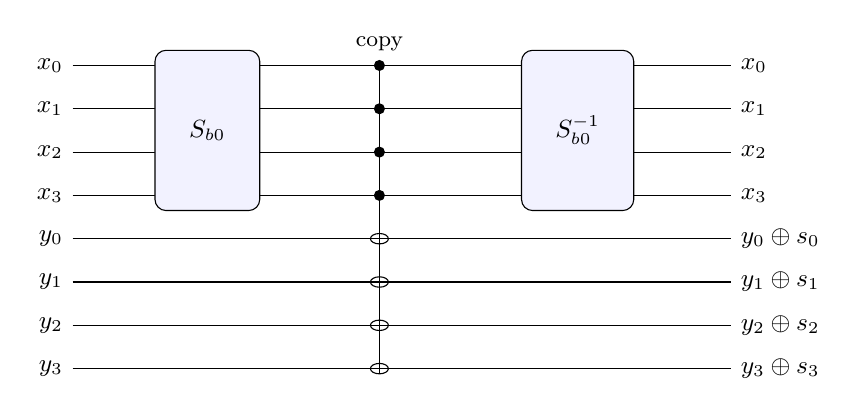
\begin{tikzpicture}[x=0.95cm,y=0.55cm,>=Latex,every node/.style={font=\small}]
% wires
\foreach \i/\lab in {0/{x_0},1/{x_1},2/{x_2},3/{x_3},4/{y_0},5/{y_1},6/{y_2},7/{y_3}}{
  \draw (0,-\i) -- (8.8,-\i);
  \node[left] at (0,-\i) {$\lab$};
}
% S box block
\draw[fill=blue!5,rounded corners] (1.1,0.35) rectangle (2.5,-3.35);
\node at (1.8,-1.5) {$\Sb$};
% inverse block
\draw[fill=blue!5,rounded corners] (6.0,0.35) rectangle (7.5,-3.35);
\node at (6.75,-1.5) {$\Sb^{-1}$};
% cnot columns
\foreach \r/\t in {0/4,1/5,2/6,3/7}{
  \fill (4.1,-\r) circle (2pt);
  \draw (4.1,-\r) -- (4.1,-\t);
  \draw (4.1,-\t) circle (0.12);
  \draw (4.1,-\t-0.12) -- (4.1,-\t+0.12);
  \draw (3.98,-\t) -- (4.22,-\t);
}
\node[font=\footnotesize] at (4.1,0.5) {copy};
\node[right] at (8.8,0) {$x_0$};
\node[right] at (8.8,-1) {$x_1$};
\node[right] at (8.8,-2) {$x_2$};
\node[right] at (8.8,-3) {$x_3$};
\node[right] at (8.8,-4) {$y_0\oplus s_0$};
\node[right] at (8.8,-5) {$y_1\oplus s_1$};
\node[right] at (8.8,-6) {$y_2\oplus s_2$};
\node[right] at (8.8,-7) {$y_3\oplus s_3$};
\end{tikzpicture}
\caption{Clean reversible implementation of the WARP Feistel nonlinear primitive. The $x$ register is transformed by $\Sb$, the four logical S-box bits are XORed into $y$ by four CNOTs, and $\Sb^{-1}$ restores $x$. The construction therefore realizes $\ket{x}\ket{y}\mapsto\ket{x}\ket{y\oplus S(x)}$ without a clean ancilla.}
\label{fig:sxor_circuit}
\end{figure}

\subsection{Key addition, constants, and permutation}
Because the key register is quantum in the Grover oracle, each key-bit XOR is implemented by a CNOT from the corresponding key qubit to the state qubit. WARP has no expanded-key state: the two 64-bit halves of the master key are selected alternately, so no additional round-key register is required.

Round constants are classical and therefore require only X gates. The nibble permutation is implemented as a logical wire map. At the block level, one reversible WARP round consists of 16 parallel Feistel S-XOR branches, quantum key addition from the active 64-bit key half, two classical round-constant nibble injections, and the fixed logical permutation (omitted in the final round). If the 32-nibble permutation were explicitly realized over an all-to-all architecture using unrestricted nibble transpositions, its two 16-cycles would require 30 nibble swaps, i.e., 120 bit-SWAPs or 360 CNOT equivalents per shuffle. We do not include this artificial logical routing overhead in the baseline circuit.


\subsection{One round and the complete cipher}
The 16 Feistel branches of one WARP round are independent before the permutation and can be processed in parallel. Every round uses 128 Toffoli gates and 256 CNOTs, plus $64+w_r$ X gates, where
\begin{equation}
    w_r = \HW(RC_0^{(r)})+\HW(RC_1^{(r)}), \qquad 1\le w_r\le 6.
\end{equation}
The total round cost therefore ranges from 449 to 454 NCT gates, with weighted full depth 65.

\begin{table}[t]
\centering
\caption{Logical resource counts for the reversible WARP-128 baseline. The permutation is treated as virtual wire relabeling.}
\label{tab:warp_resources}
\begin{tabular}{lrrrrrr}
\toprule
Component & Qubits & X & CNOT & CCX & NCT total & Weighted depth\\
\midrule
One round & 256 & $64+w_r$ & 256 & 128 & $448+w_r$ & 65\\
Full 41 rounds & 256 & 2,763 & 10,496 & 5,248 & 18,507 & 1,435\\
\bottomrule
\end{tabular}
\end{table}

The complete 41-round logical circuit requires 256 qubits (128 state and 128 key), no clean ancilla, and 18,507 NCT gates. The simple exact-Toffoli accounting gives
\begin{equation}
    T_E = 7\times 5{,}248 = 36{,}736
\end{equation}
pre-optimization $T$ gates for one encryption. Interestingly, the full weighted depth is 1,435 rather than $41\times65=2,665$ because the GFN permutation moves the critical path between wires and allows inter-round scheduling overlap.

\subsection{Correctness verification}
The reversible implementation was tested at three levels. First, 1,000 randomly generated standalone rounds were compared with an independent classical WARP implementation. Second, the complete reversible circuit reproduced all three official WARP test vectors. Third, 100 random full-cipher encryptions were compared against the independent classical implementation. Reversing the complete NCT gate list restored both the state and the quantum key registers exactly.

\begin{table}[t]
\centering
\caption{Two official same-key WARP vectors used for the known-plaintext Grover experiments. A third official vector is included in the regression suite.}
\label{tab:vectors}
\small
\begin{tabular}{c@{\;}l}
\toprule
Key & \texttt{0123456789ABCDEFFEDCBA9876543210}\\
\midrule
$P_1$ & \texttt{0123456789ABCDEFFEDCBA9876543210}\\
$C_1$ & \texttt{24CE0A8EFD9F32DE529D5FDF45703A8D}\\
\addlinespace
$P_2$ & \texttt{00112233445566778899AABBCCDDEEFF}\\
$C_2$ & \texttt{923C64F92827EE62B9667DD2548FB12C}\\
\bottomrule
\end{tabular}
\end{table}
\FloatBarrier

\section{Known-Plaintext Grover Oracles}

\subsection{One-pair phase oracle}
For a known pair $(P_1,C_1)$, define
\begin{equation}
    f_1(K)=[E_K(P_1)=C_1].
\end{equation}
The phase oracle is implemented as
\begin{equation}
U_E\;\rightarrow\;\textsf{Normalize}(C_1)\;\rightarrow\;\mathrm{MCZ}_{128}\;\rightarrow\;\textsf{Denormalize}\;\rightarrow\;U_E^{-1}.
\end{equation}
A 128-bit equality phase uses 125 clean work ancillas and a clean AND ladder containing 251 Toffoli gates. The resulting one-pair phase oracle uses 381 qubits and 10,747 Toffolis.

\subsection{Exact identifiability law under the ideal-cipher model}
\label{subsec:identifiability}
Let the block size be $b$, the key size be $k$, and let
\[
(P_1,C_1),\ldots,(P_r,C_r),\qquad C_i=E_{K^\star}(P_i),
\]
be $r$ distinct known plaintext/ciphertext pairs generated under the unknown master key $K^\star$.  Because encryption under a fixed key is a permutation, distinct plaintexts have distinct target ciphertexts.  Write
\begin{equation}
    (2^b)_r=2^b(2^b-1)\cdots(2^b-r+1)
\end{equation}
for the falling factorial.

\begin{proposition}[Wrong-key pass probability]
Under the ideal-cipher model, in which the permutations associated with distinct keys are independent and uniformly random, a fixed wrong key $K\neq K^\star$ satisfies all $r$ pairs with probability
\begin{equation}
    p_r=\frac{1}{(2^b)_r}.
    \label{eq:wrong_key_pass}
\end{equation}
\end{proposition}
\begin{proof}
The first prescribed mapping occurs with probability $1/2^b$.  Conditional on it, only $2^b-1$ output points remain for the second distinct plaintext, then $2^b-2$ for the third, and so on.  Multiplying these conditional probabilities gives Eq.~\eqref{eq:wrong_key_pass}.
\end{proof}

\begin{proposition}[False-key distribution]
Let $W_r$ denote the number of wrong keys satisfying all $r$ pairs.  Under the same ideal-cipher assumptions,
\begin{equation}
    W_r\sim\operatorname{Binomial}\!\left(2^k-1,\frac{1}{(2^b)_r}\right),
    \label{eq:falsekey_binomial}
\end{equation}
so
\begin{equation}
    \E[W_r]=\frac{2^k-1}{(2^b)_r},
    \label{eq:wrongkeys}
\end{equation}
and the probability that the supplied data uniquely identify the true key is
\begin{equation}
    \Prb[W_r=0]=
    \left(1-\frac{1}{(2^b)_r}\right)^{2^k-1}.
    \label{eq:unique_key_probability}
\end{equation}
For $r\ll2^b$, Eq.~\eqref{eq:wrongkeys} reduces to the familiar approximation $2^{k-rb}$.
\end{proposition}

\begin{corollary}[WARP-128 parameters under the ideal-cipher model]
For WARP, $k=b=128$.  With one pair,
\begin{equation}
    \E[W_1]=1-2^{-128}
\end{equation}
and
\begin{equation}
    \Prb[W_1=0]=
    \left(1-2^{-128}\right)^{2^{128}-1}\approx e^{-1}.
\end{equation}
Thus the probability of at least one additional wrong survivor is approximately $1-e^{-1}\approx0.63212$.  With two distinct pairs,
\begin{equation}
    \E[W_2]
    =\frac{2^{128}-1}{2^{128}(2^{128}-1)}
    =2^{-128},
\end{equation}
and
\begin{equation}
    \Prb[W_2=0]
    =\left(1-\frac{1}{2^{128}(2^{128}-1)}\right)^{2^{128}-1}
    \approx 1-2^{-128}.
\end{equation}
\end{corollary}

This distinction also changes how Grover success should be interpreted.  If $M=1+W_r$ keys satisfy the supplied data and the oracle marks all of them symmetrically, then with
\begin{equation}
    \theta_M=\arcsin\sqrt{\frac{M}{2^k}},
\end{equation}
the aggregate marked-state probability is
\begin{equation}
    P_{\rm mark}(j\mid M)=
    \sin^2\!\bigl((2j+1)\theta_M\bigr),
    \label{eq:aggregate_marked_probability}
\end{equation}
whereas each particular marked key has probability
\begin{equation}
    P_{\rm one}(j\mid M)=\frac{1}{M}P_{\rm mark}(j\mid M).
    \label{eq:specific_marked_probability}
\end{equation}
Consequently, when $M>1$, a one-pair oracle solves ``find a key consistent with the observed mapping''; it cannot identify which satisfying key was historically used.  Multi-pair conjunction is therefore part of the attack definition for unique-master-key recovery, not merely a circuit-design refinement.

\subsection{Cross-cipher extension and validation: Mini-AES and S-AES}
\label{subsec:cross_cipher_validation}
The ideal-permutation law above is cipher-agnostic.  To check that the single-pair phenomenon motivating the WARP oracle is not peculiar to one construction, we independently implemented Mini-AES and S-AES and exhaustively evaluated all $2^{16}$ candidate keys for selected known pairs.  Table~\ref{tab:cross_cipher_validation} reports the exact satisfying sets.

\begin{table}[H]
\centering
\caption{Exhaustive $2^{16}$-key validation of one-pair multiplicity and two-pair uniqueness in two independent 16-bit SPNs.}
\label{tab:cross_cipher_validation}
\begin{tabular}{lrrrr}
\toprule
Cipher & True key & $M(P_1,C_1)$ & $M(P_2,C_2)$ & $M(\text{both})$\\
\midrule
Mini-AES & \texttt{C3F0} & 3 & 3 & 1\\
S-AES & \texttt{4AF5} & 3 & 2 & 1\\
\bottomrule
\end{tabular}
\end{table}

For Mini-AES, the two satisfying-key sets are
\begin{align}
\mathcal{K}^{\rm Mini}_1
&=\{\mathtt{98DD},\mathtt{C3F0},\mathtt{E873}\},
& (P_1,C_1)&=(\mathtt{9C63},\mathtt{72C6}),\\
\mathcal{K}^{\rm Mini}_2
&=\{\mathtt{C3F0},\mathtt{DBEA},\mathtt{F330}\},
& (P_2,C_2)&=(\mathtt{0000},\mathtt{7BBA}),
\end{align}
with $\mathcal{K}^{\rm Mini}_1\cap\mathcal{K}^{\rm Mini}_2=\{\mathtt{C3F0}\}$.  For S-AES,
\begin{align}
\mathcal{K}^{\rm SAES}_1
&=\{\mathtt{4AF5},\mathtt{C5A1},\mathtt{DA76}\},
& (P_1,C_1)&=(\mathtt{D728},\mathtt{24EC}),\\
\mathcal{K}^{\rm SAES}_2
&=\{\mathtt{4AF5},\mathtt{5A70}\},
& (P_2,C_2)&=(\mathtt{0000},\mathtt{52B1}),
\end{align}
with $\mathcal{K}^{\rm SAES}_1\cap\mathcal{K}^{\rm SAES}_2=\{\mathtt{4AF5}\}$.  Thus the first tested pair has three satisfying keys in both ciphers, but a second pair reduces the common set to the intended key.

We additionally fixed a 16-plaintext panel in advance and, for each plaintext and cipher, computed the complete 65,536-key ciphertext-occupancy spectrum. Against a 20,000-sample random-mapping Monte Carlo calibration, the smallest empirical upper-tail $p$-values were approximately $0.0712$ for Mini-AES and $0.0136$ for S-AES. Treating the full cross-cipher panel as 32 pre-declared tests gives the conservative Bonferroni threshold $0.05/32=0.0015625$, so neither minimum survives this correction. These finite-panel experiments do not prove ideal-cipher behavior, and the Monte Carlo tests are used only as a descriptive model check; they provide no corrected evidence that the observed occupancy spectra depart from the stated random-mapping baseline. The same one-pair versus multi-pair distinction is observable internally in Toy-WARP-8 in Section~\ref{sec:toywarp8}.

\subsection{Two-pair AND oracle}
For unique-key recovery we therefore use
\begin{equation}
    f_2(K)=[E_K(P_1)=C_1]\land[E_K(P_2)=C_2].
    \label{eq:two_pair_pred}
\end{equation}
It is essential that the two predicates are combined by logical AND. Sequentially applying two independent phase flips would mark $f_1\oplus f_2$, which is not the desired predicate.

We implement three two-pair designs.
\begin{itemize}
    \item \textbf{Direct wide AND:} two 128-bit state registers are encrypted under the same key and a single 256-bit equality condition is phase-marked. This is the gate-efficient design.
    \item \textbf{Two equality flags:} each equality is compressed into a one-qubit flag and a CZ on the two flags marks the joint predicate. This reduces width at a small gate penalty.
    \item \textbf{Compact recomputation:} one state register and one equality flag are used. The first encryption is recomputed later to erase the stored flag. This nearly matches the one-pair width but increases gate count and depth.
\end{itemize}

\begin{figure}[tbp]
\centering
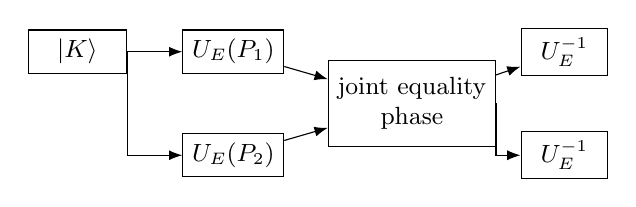
\begin{tikzpicture}[>=Latex, node distance=0.95cm and 0.7cm, every node/.style={font=\small}]
\node (k) [draw, minimum width=1.25cm] {$\ket{K}$};
\node (e1) [draw, right=of k, minimum width=1.1cm] {$U_E(P_1)$};
\node (e2) [draw, below=0.75cm of e1, minimum width=1.1cm] {$U_E(P_2)$};
\node (cmp) [draw, right=1.2cm of $(e1)!0.5!(e2)$, minimum width=1.7cm, minimum height=1.1cm, align=center] {joint equality\\phase};
\node (u1) [draw, right=1.2cm of e1, xshift=1.8cm, minimum width=1.1cm] {$U_E^{-1}$};
\node (u2) [draw, right=1.2cm of e2, xshift=1.8cm, minimum width=1.1cm] {$U_E^{-1}$};
\draw[->] (k) -- (e1);
\draw[->] (k.east) |- (e2.west);
\draw[->] (e1) -- (cmp);
\draw[->] (e2) -- (cmp);
\draw[->] (cmp) -- (u1);
\draw[->] (cmp.east) |- (u2.west);
\end{tikzpicture}
\caption{Two-pair WARP phase oracle. The candidate key controls two full WARP encryptions for independent known plaintexts. A single joint equality predicate flips the phase only when both computed ciphertexts match their targets; both encryption workspaces are then uncomputed.}
\label{fig:two_pair_oracle}
\end{figure}

\begin{table}[t]
\centering
\caption{Logical resources for the phase-oracle constructions. The $T$-count is the transparent pre-optimization value $7\times\#\mathrm{CCX}$.}
\label{tab:oracle_resources}
\small
\begin{tabular}{lrrrrr}
\toprule
Construction & Qubits & CCX & Total gates & Weighted depth & $T$ count\\
\midrule
One pair & 381 & 10,747 & 37,383 & 4,629 & 75,229\\
Two pairs, wide AND & 637 & 21,499 & 74,779 & 7,381 & 150,493\\
Two pairs, two flags & 512 & 22,004 & 75,525 & 9,958 & 154,028\\
Two pairs, compact & 383 & 32,247 & 112,289 & 13,929 & 225,729\\
\bottomrule
\end{tabular}
\end{table}

\subsection{Complete Grover-iteration costs}
Adding a standard 128-bit diffuser yields the resource counts in Table~\ref{tab:iteration_resources}; the resulting iteration structure is summarized in the clean register-level circuit of Figure~\ref{fig:full_grover_circuit}. For the two-pair wide construction, one iteration contains 21,750 Toffolis and therefore a baseline
\begin{equation}
    T_{\mathrm{iter}}=152{,}250.
\end{equation}
Under the unique-key model $M=1$, the iteration count is approximately
\begin{equation}
    R_G \approx \frac{\pi}{4}2^{64}, \qquad \log_2 R_G\approx63.6515.
\end{equation}
The corresponding pre-optimization logical $T$ workload is
\begin{equation}
    R_G\,T_{\mathrm{iter}} \approx 2.21\times10^{24}\approx2^{80.87}.
    \label{eq:total_t}
\end{equation}
This is a logical circuit workload rather than a physical time estimate.

\begin{table}[t]
\centering
\caption{One complete Grover iteration: phase oracle plus 128-bit diffuser.}
\label{tab:iteration_resources}
\small
\begin{tabular}{lrrrrr}
\toprule
Construction & Qubits & CCX & Total gates & Weighted depth & $T$ count\\
\midrule
One pair & 381 & 10,998 & 38,148 & 6,355 & 76,986\\
Two pairs, wide AND & 637 & 21,750 & 75,544 & 9,109 & 152,250\\
Two pairs, two flags & 512 & 22,255 & 76,290 & 11,684 & 155,785\\
Two pairs, compact & 383 & 32,498 & 113,054 & 15,655 & 227,486\\
\bottomrule
\end{tabular}
\end{table}

\begin{figure}[tbp]
\centering
\resizebox{0.96\textwidth}{!}{%
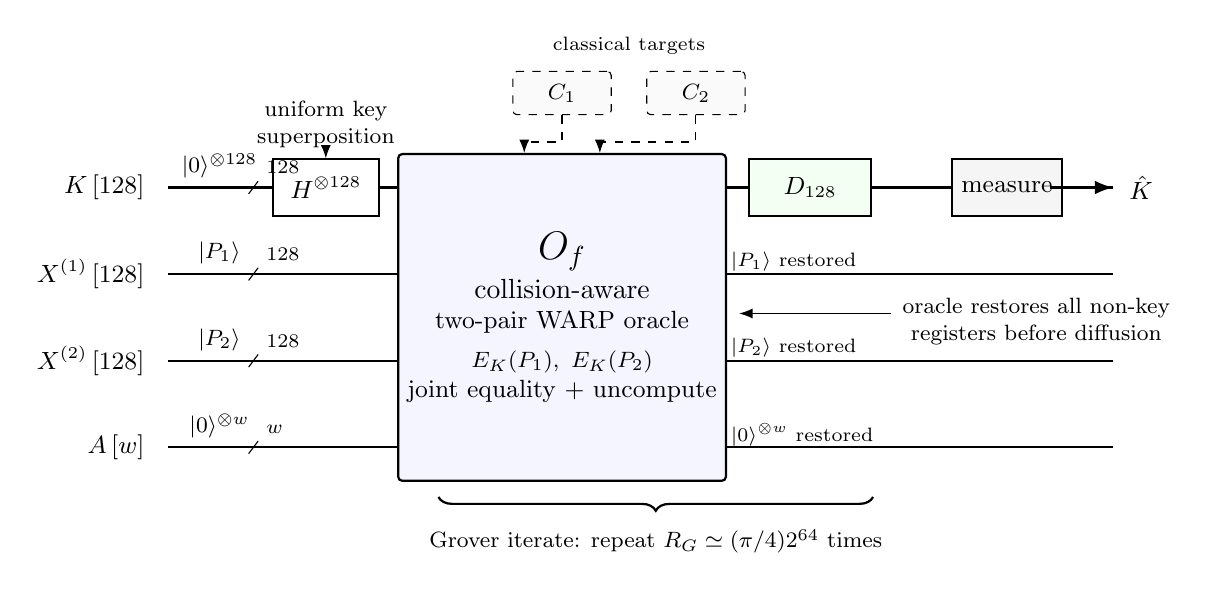
\begin{tikzpicture}[x=1cm,y=1cm,>=Latex,
  every node/.style={font=\small},
  block/.style={draw,thick,fill=white,minimum height=0.72cm,align=center},
  oracle/.style={draw,thick,fill=blue!4,rounded corners=1.5pt,align=center},
  diff/.style={draw,thick,fill=green!5,minimum width=1.55cm,minimum height=0.72cm,align=center},
  meas/.style={draw,thick,fill=gray!8,minimum width=1.10cm,minimum height=0.72cm,align=center},
  ctarget/.style={draw,dashed,rounded corners=1.5pt,fill=gray!4,minimum width=1.25cm,minimum height=0.55cm,align=center,font=\footnotesize}]

% y coordinates for grouped registers
\def\yk{3.15}
\def\ypa{2.05}
\def\ypb{0.95}
\def\yw{-0.15}

% register wires
\draw[thick] (0,\yk) -- (12.0,\yk);
\draw[thick] (0,\ypa) -- (12.0,\ypa);
\draw[thick] (0,\ypb) -- (12.0,\ypb);
\draw[thick] (0,\yw) -- (12.0,\yw);

% register labels
\node[anchor=east] at (-0.18,\yk) {$K\,[128]$};
\node[anchor=east] at (-0.18,\ypa) {$X^{(1)}\,[128]$};
\node[anchor=east] at (-0.18,\ypb) {$X^{(2)}\,[128]$};
\node[anchor=east] at (-0.18,\yw) {$A\,[w]$};

% initialization labels
\node[anchor=south,font=\footnotesize] at (0.65,\yk) {$\ket{0}^{\otimes128}$};
\node[anchor=south,font=\footnotesize] at (0.65,\ypa) {$\ket{P_1}$};
\node[anchor=south,font=\footnotesize] at (0.65,\ypb) {$\ket{P_2}$};
\node[anchor=south,font=\footnotesize] at (0.65,\yw) {$\ket{0}^{\otimes w}$};

% Hadamard preparation on key register
\node[block,minimum width=1.35cm] (H) at (2.0,\yk) {$H^{\otimes128}$};

% main oracle spanning all quantum registers
\node[oracle,minimum width=3.00cm,minimum height=4.15cm] (Of) at (5.0,1.50)
 {\Large $O_f$\\[2pt]\normalsize collision-aware\\two-pair WARP oracle\\[3pt]\footnotesize $E_K(P_1),\ E_K(P_2)$\\joint equality + uncompute};

% classical ciphertext targets
\node[ctarget] (C1) at (5.0,4.35) {$C_1$};
\node[ctarget] (C2) at (6.70,4.35) {$C_2$};
\draw[dashed,->] (C1.south) -- ++(0,-0.34) -| ([xshift=-0.48cm]Of.north);
\draw[dashed,->] (C2.south) -- ++(0,-0.34) -| ([xshift=0.48cm]Of.north);
\node[font=\scriptsize,anchor=south] at (5.85,4.72) {classical targets};

% diffuser on key only
\node[diff] (D) at (8.15,\yk) {$D_{128}$};

% measurement on key only
\node[meas] (M) at (10.65,\yk) {measure};
\draw[->,thick] (11.20,\yk) -- (12.0,\yk);
\node[anchor=west] at (12.08,\yk) {$\hat K$};

% restored-state labels
\node[font=\scriptsize,anchor=west] at (7.02,\ypa+0.16) {$\ket{P_1}$ restored};
\node[font=\scriptsize,anchor=west] at (7.02,\ypb+0.16) {$\ket{P_2}$ restored};
\node[font=\scriptsize,anchor=west] at (7.02,\yw+0.16) {$\ket{0}^{\otimes w}$ restored};

% repeat brace under oracle + diffuser only
\draw[decorate,decoration={brace,amplitude=5pt,mirror},thick]
      (3.43,-0.78) -- (8.95,-0.78)
      node[midway,below=8pt,font=\footnotesize]
      {Grover iterate: repeat $R_G\simeq(\pi/4)2^{64}$ times};

% clean explanatory annotations
\node[font=\footnotesize,align=center] at (2.0,3.95)
 {uniform key\\superposition};
\draw[->] (2.0,3.63) -- (2.0,3.52);

\node[font=\footnotesize,align=center,anchor=west] at (9.20,1.45)
 {oracle restores all non-key\\registers before diffusion};
\draw[->] (9.18,1.55) -- (7.25,1.55);

% bus-size slash markers
\foreach \yy in {\yk,\ypa,\ypb,\yw}{
  \draw (1.02,\yy-0.08) -- (1.14,\yy+0.08);
}
\node[font=\scriptsize,anchor=south west] at (1.12,\yk+0.05) {128};
\node[font=\scriptsize,anchor=south west] at (1.12,\ypa+0.05) {128};
\node[font=\scriptsize,anchor=south west] at (1.12,\ypb+0.05) {128};
\node[font=\scriptsize,anchor=south west] at (1.12,\yw+0.05) {$w$};

\end{tikzpicture}%
}
\caption{Register-level Grover circuit used for collision-aware known-plaintext key search on WARP-128. The 128-bit key register is prepared in uniform superposition by $H^{\otimes128}$. The oracle $O_f$ evaluates full WARP encryption for the two known plaintexts, compares the resulting ciphertexts with the classical targets $C_1$ and $C_2$, applies the phase mark only when both comparisons succeed, and uncomputes the state and workspace registers. The diffuser $D_{128}$ acts only on the key register. The oracle--diffuser pair is repeated approximately $R_G\simeq(\pi/4)2^{64}$ times in the unique-key model before the key register is measured.}
\label{fig:full_grover_circuit}
\end{figure}

\subsection{Depth-oriented equality trees and parallel key fanout}
\label{subsec:depth_oracle}
The linear clean-ancilla multi-controlled phase used above uses one fewer Toffoli than the balanced construction described next, but it creates a long serial dependency chain. For $n=2^m$ condition bits, we therefore also implement a balanced AND tree. Pairwise ANDs are computed into clean ancillas until two root bits remain, a CZ gate applies the phase, and the tree is uncomputed. This construction uses
\begin{equation}
    n-2\ \text{clean ancillas},\qquad 2(n-2)\ \text{CCX gates},
\end{equation}
and has Toffoli-layer depth
\begin{equation}
    2(m-1).
\end{equation}
Thus a 256-bit joint equality test uses 254 clean ancillas, 508 Toffolis, and only 14 Toffoli layers. Relative to the ladder comparator, this costs one additional ancilla and one additional Toffoli but substantially reduces depth.

We also introduce a depth-oriented two-pair architecture with a coherent copy of the 128-bit key register. The map
\begin{equation}
    \sum_k \alpha_k\ket{k}\ket{0}\longmapsto
    \sum_k \alpha_k\ket{k}\ket{k}
\end{equation}
is implemented by 128 CNOTs. This is computational-basis fanout rather than cloning an arbitrary unknown quantum state. The copied key controls the second WARP encryption, so the two encryption circuits act on disjoint state/key wires and can be scheduled in parallel; after inverse encryption, the key copy is uncomputed by the inverse fanout.

Table~\ref{tab:ft_depth_models} compares the resulting constructions. The balanced comparator alone lowers the complete-iteration Toffoli-layer depth from 1,156 to 678. Adding coherent key fanout lowers it further to 358, while the $T$-count changes only from 152,250 to 152,264. The price is width: 638 logical qubits for the balanced shared-key version and 766 for the parallel-key version.

\begin{figure}[tbp]
\centering
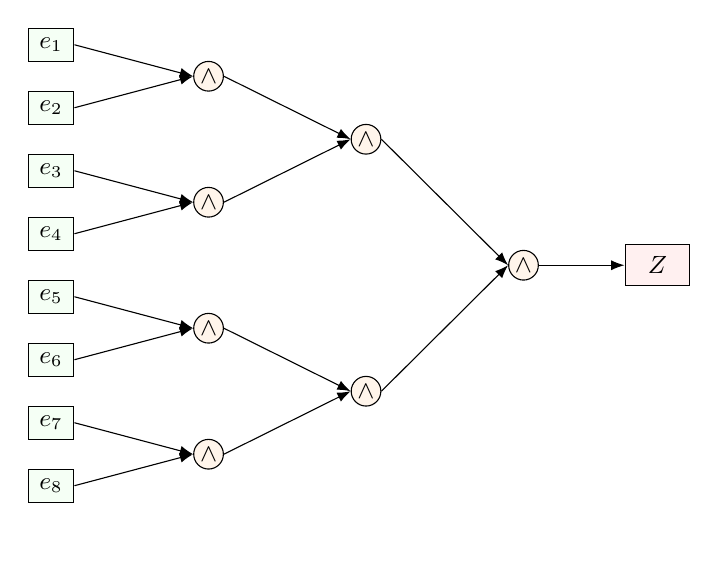
\begin{tikzpicture}[>=Latex,every node/.style={font=\small},
bit/.style={draw, minimum width=0.58cm, minimum height=0.42cm, fill=green!4},
andnode/.style={draw, circle, inner sep=1pt, fill=orange!8},
phase/.style={draw, minimum width=0.82cm, minimum height=0.52cm, fill=red!6}]
% leaves
\node[bit] (b1) at (0,0) {$e_1$};
\node[bit] (b2) at (0,-0.8) {$e_2$};
\node[bit] (b3) at (0,-1.6) {$e_3$};
\node[bit] (b4) at (0,-2.4) {$e_4$};
\node[bit] (b5) at (0,-3.2) {$e_5$};
\node[bit] (b6) at (0,-4.0) {$e_6$};
\node[bit] (b7) at (0,-4.8) {$e_7$};
\node[bit] (b8) at (0,-5.6) {$e_8$};
% first level
\node[andnode] (c1) at (2,-0.4) {$\wedge$};
\node[andnode] (c2) at (2,-2.0) {$\wedge$};
\node[andnode] (c3) at (2,-3.6) {$\wedge$};
\node[andnode] (c4) at (2,-5.2) {$\wedge$};
\draw[->] (b1.east) -- (c1.west); \draw[->] (b2.east) -- (c1.west);
\draw[->] (b3.east) -- (c2.west); \draw[->] (b4.east) -- (c2.west);
\draw[->] (b5.east) -- (c3.west); \draw[->] (b6.east) -- (c3.west);
\draw[->] (b7.east) -- (c4.west); \draw[->] (b8.east) -- (c4.west);
% second level
\node[andnode] (d1) at (4,-1.2) {$\wedge$};
\node[andnode] (d2) at (4,-4.4) {$\wedge$};
\draw[->] (c1.east) -- (d1.west); \draw[->] (c2.east) -- (d1.west);
\draw[->] (c3.east) -- (d2.west); \draw[->] (c4.east) -- (d2.west);
% root and phase
\node[andnode] (r) at (6,-2.8) {$\wedge$};
\draw[->] (d1.east) -- (r.west); \draw[->] (d2.east) -- (r.west);
\node[phase] (z) at (7.7,-2.8) {$Z$};
\draw[->] (r.east) -- (z.west);
\node[align=center,font=\footnotesize] at (6,-6.2) {\shortstack{}};
\end{tikzpicture}
\caption{Balanced equality-tree comparator (eight-leaf schematic). In the 256-bit two-pair oracle, the same binary-tree pattern reduces all ciphertext-equality bits to a logarithmic-depth phase condition and is then exactly uncomputed. This exchanges one extra Toffoli and one extra ancilla relative to the ladder construction for a much smaller Toffoli-layer depth.}
\label{fig:balanced_tree}
\end{figure}

\begin{table}[t]
\centering
\caption{Fault-tolerant depth models for WARP encryption and the principal two-pair Grover iterations. FT-A uses a seven-$T$, $T$-depth-three exact Toffoli without decomposition ancillas; FT-B uses the seven-$T$, $T$-depth-one, four-ancilla Toffoli. The FT-B width is a conservative upper bound based on the peak number of parallel CCX gates.}
\label{tab:ft_depth_models}
\scriptsize
\begin{tabular}{lrrrrrr}
\toprule
Construction & Logical Q & $T$ count & $D_{\rm CCX}$ & $T$-depth A & $T$-depth B & FT-B Q upper\\
\midrule
WARP encryption & 256 & 36,736 & 168 & 504 & 168 & 384\\
Two-pair ladder iteration & 637 & 152,250 & 1,156 & 3,468 & 1,156 & 829\\
Two-pair balanced iteration & 638 & 152,264 & 678 & 2,034 & 678 & 1,150\\
Two-pair parallel+balanced & 766 & 152,264 & 358 & 1,074 & 358 & 1,278\\
\bottomrule
\end{tabular}
\end{table}

These numbers reinforce the width--depth lesson observed in prior Grover-oracle and lightweight-cipher resource studies~\cite{Jaques2020,Rahman2022}: a nearly unchanged non-Clifford gate count can hide a large design space in logical width and $T$-depth.
\FloatBarrier

\section{Executable Known-Plaintext Grover Experiments}

Dense statevector simulation of the full 256-qubit encryption circuit, let alone the 381--766-qubit Grover oracles, is classically infeasible. To obtain an executable experiment without defining an artificial reduced cipher, we keep the complete 41-round WARP function and restrict only $u$ master-key bits to be unknown. The remaining key bits are fixed to the official test-vector key. For every candidate in the $2^u$ subspace, the marked predicate is evaluated using the actual reversible 18,507-gate WARP circuit; Grover amplitudes are then simulated exactly over the $u$-qubit candidate register.

\subsection{Exact sparse-simulation principle}
The restricted-key experiment admits an exact sparse simulation because the WARP circuit is a reversible classical permutation. Let $U$ be any circuit over X, CNOT, and Toffoli gates and let
\begin{equation}
    \ket{\psi}=\sum_{a\in A}\alpha_a\ket{a},
    \qquad |A|=2^u.
\end{equation}
Since $U$ permutes computational-basis states, there exists a bijection $\pi_U$ such that
\begin{equation}
    U\ket{\psi}=\sum_{a\in A}\alpha_a\ket{\pi_U(a)}.
\end{equation}
Therefore the support cardinality is preserved exactly:
\begin{equation}
    \bigl|\operatorname{supp}(U\ket{\psi})\bigr|=2^u.
    \label{eq:sparse_support}
\end{equation}
In our construction the quantum key register is retained, so distinct candidate keys remain distinct basis branches throughout all 41 rounds. The phase predicate does not enlarge the support, and after uncomputation the state returns to the $u$-qubit candidate subspace before the diffuser.

Consequently, the marked set can be generated in $O(2^u G_E)$ reversible-gate operations, where $G_E=18{,}507$ is the verified WARP encryption gate count, and Grover amplitudes can be simulated in $O(2^u)$ memory rather than allocating a dense $2^{256}$ statevector. The subsequent amplitude simulation costs $O(R2^u)$ for $R$ Grover iterations. We explicitly verified support preservation for all $2^8=256$ candidate branches through the complete 41-round circuit. This is an exact property of the restricted-key experiment, not an approximation; it does not make the full $u=128$ simulation practical.

For $u\in\{8,10,12\}$ and the least-significant unknown-key subspaces considered in our experiments, both the one-pair and two-pair predicates have one marked candidate. Table~\ref{tab:exec} summarizes the ideal amplitude-amplification results.

\begin{table}[t]
\centering
\caption{Executable Grover experiments using the full 41-round WARP predicate and a restricted unknown-key subspace.}
\label{tab:exec}
\begin{tabular}{rrrrr}
\toprule
Unknown bits $u$ & $N$ & $M$ & Optimal $j$ & Success probability\\
\midrule
8 & 256 & 1 & 12 & 0.9999470\\
10 & 1,024 & 1 & 25 & 0.9994612\\
12 & 4,096 & 1 & 50 & 0.9999453\\
\bottomrule
\end{tabular}
\end{table}

For $u=8$, the numerical statevector result after 12 iterations is
\begin{equation}
    P_{\mathrm{num}}=0.9999470421032738,
\end{equation}
while Eq.~\eqref{eq:grover_success} gives
\begin{equation}
    P_{\mathrm{theory}}=0.9999470421032736.
\end{equation}
The difference is at machine precision. In a 1,024-shot seeded simulation, the correct candidate was observed in all 1,024 measurements. The experiment demonstrates the key-recovery logic and amplitude dynamics; it is not a claim that the full 128-bit search can be simulated or executed on current hardware.


\section{Executable Toy-WARP-8 Full-Key Recovery}
\label{sec:toywarp8}

The preceding experiment preserves the complete 41-round WARP predicate but restricts the unknown-key subspace.  To complement it with a literal end-to-end Grover circuit over an entire key space, we additionally define an explicitly reduced demonstrator, \emph{Toy-WARP-8}.  This construction is a simulation vehicle only: it is \emph{not} a reduced-round security claim for WARP-128 and its results are not extrapolated to the security of the standardized cipher.  Its role is analogous to the reduced executable instances used in small-cipher quantum studies~\cite{Kiran2026}, while keeping the WARP nonlinear primitive and Feistel update visible.

\subsection{Definition and exhaustive reversible verification}
Toy-WARP-8 has an 8-bit block and an 8-bit key,
\begin{equation}
    X=X_0\|X_1,\qquad K=K_0\|K_1,
\end{equation}
where each component is a nibble.  It retains the exact WARP/MIDORI $S_{b0}$ S-box.  In zero-based round $r$,
\begin{equation}
    X_1\leftarrow X_1\oplus S_{b0}(X_0)\oplus K_{r\bmod 2}\oplus RC_r,
    \label{eq:toywarp_round}
\end{equation}
followed by the natural two-branch Feistel swap except after the final round.  We use eight rounds.  For this one-branch toy state, the two WARP LFSR-derived round-constant nibbles are combined as $RC_r=RC0_r\oplus RC1_r$, giving
\begin{equation}
    (RC_0,\ldots,RC_7)=(4,\mathrm{C},\mathrm{D},\mathrm{F},\mathrm{B},3,7,\mathrm{B}).
\end{equation}

The reversible implementation uses 16 logical qubits: eight state qubits and eight master-key qubits.  It requires no clean ancilla and contains 53 X, 128 CNOT, and 64 Toffoli gates, for 245 NCT gates and a transparent pre-optimization $T$ count of 448.  We exhaustively verified that every one of the $2^8$ keys induces a permutation of the 256 plaintexts and that the reversible gate circuit agrees with the classical implementation on all
\begin{equation}
    2^8\cdot2^8=65{,}536
\end{equation}
key/plaintext evaluations.

\subsection{One-pair recovery, collisions, and two-pair disambiguation}
For the test vector
\begin{equation}
    K=\mathtt{C6},\qquad P=\mathtt{00},\qquad C=\mathtt{CE},
\end{equation}
full enumeration of the 256-key space gives the unique marked set
\begin{equation}
    \mathcal{M}_1=\{\mathtt{C6}\}.
\end{equation}
Thus $N=256$ and $M=1$.  The first Grover maximum occurs at $j=12$, with exact probability
\begin{equation}
    P_{12}=0.9999470421032738.
\end{equation}

The same reduced construction also makes the single-pair collision issue directly observable.  For
\begin{equation}
    P=\mathtt{05},\qquad C=\mathtt{3F},
\end{equation}
the complete key enumeration gives
\begin{equation}
    \mathcal{M}_1=\{\mathtt{18},\mathtt{2F},\mathtt{C6}\},
\end{equation}
so Grover amplifies three valid candidate keys rather than uniquely identifying the generating key.  Adding the independent pair
\begin{equation}
    (P_2,C_2)=(\mathtt{00},\mathtt{CE})
\end{equation}
to $(P_1,C_1)=(\mathtt{05},\mathtt{3F})$ leaves only
\begin{equation}
    \mathcal{M}_2=\{\mathtt{C6}\}.
\end{equation}
Across all 65,536 choices of true key and plaintext, the empirical mean number of one-pair marked keys is 1.92834, compared with the ideal-cipher conditional baseline $1+255/256\approx1.99609$. We report this as a descriptive diagnostic only: the 65,536 values are highly dependent because they are generated by one fixed toy construction, so this mean is not used as an independence-based goodness-of-fit test. Its relevant qualitative message is simply that one-pair multiplicity is common in the reduced domain; structural claims would require a separately specified statistical test.

\subsection{Actual Qiskit/Aer end-to-end Grover execution}
\label{subsec:toywarp_qiskit}
We implemented the complete Toy-WARP-8 oracle in Qiskit and executed it with Qiskit Aer.  The circuit prepares all 256 candidate keys with $H^{\otimes 8}$, performs the full eight-round reversible encryption, applies an 8-bit ciphertext equality phase test, uncomputes the encryption, applies the 8-qubit diffuser, and repeats this oracle--diffuser pair 12 times before measuring the entire key register.

In the 4,096-shot ideal run, the correct bit string
\begin{equation}
    \mathtt{11000110}=\mathtt{C6}
\end{equation}
was observed 4,095 times, while one shot returned $\mathtt{05}$.  Hence
\begin{equation}
    \widehat P_{\mathrm{Aer}}=\frac{4095}{4096}=0.9997558594,
\end{equation}
consistent with the exact ideal value $P_{12}=0.9999470421$.  Under the default ideal-run transpilation used for this experiment, the reported circuit depth was 2,127, with 2,808 CX, 1,360 CCX, 1,184 X, 24 MCX, 192 U2, 24 U1, eight H, and eight measurement operations.  These transpiled Qiskit counts are reported separately from the logical NCT resource table because the two use different compilation and gate-library conventions.

\subsection{End-to-end depolarizing-noise sweep}
\label{subsec:toywarp_noise}
We next executed a controlled Qiskit/Aer depolarizing-noise campaign. Before noisy simulation, each Grover circuit was transpiled to the basis
\[
    \{\mathrm{RZ},\mathrm{SX},X,\mathrm{CX}\}
\]
at optimization level one, so CCX and MCX operations were decomposed into one- and two-qubit basis gates. RZ was treated as virtual/noiseless; X/SX locations received one-qubit depolarizing probability $p_1$, and CX locations received two-qubit depolarizing probability $p_2$. This remains an explicitly parameterized simulator model rather than a calibrated hardware forecast.

To isolate stochastic simulation variability from compilation variability, each $j$-iteration circuit was transpiled exactly once using fixed transpiler seed 777 and then reused unchanged in every replicate. Only the Aer simulator seed was varied, using seeds 101, 202, and 303. Each replicate used 4,096 shots, so every plotted point pools
\[
    3\times4096=12{,}288
\]
shots. The depths of the fixed compiled circuits for $j=3,6,9,12$ were 3,687, 7,395, 11,103, and 14,811, respectively.

Figure~\ref{fig:toywarp_qiskit_noise} reports the pooled correct-key probabilities with 95\% Wilson intervals. The pooled simulator estimates in the zero-noise scenario for $j=3,6,9,12$ are 0.177816, 0.527507, 0.858561, and 0.999919, respectively, and agree closely with the exact Grover probabilities 0.179721, 0.527618, 0.860676, and 0.999947. Under mild noise $(p_1,p_2)=(10^{-5},10^{-4})$, the corresponding pooled probabilities are 0.139730, 0.358236, 0.478678, and 0.523438. Under the stronger setting $(10^{-4},10^{-3})$, they fall to 0.027588, 0.023519, 0.020264, and 0.014323. Thus increasing circuit length continues to improve success in the mild regime up to the tested $j=12$ point, but under stronger noise the accumulated error dominates and the success probability decreases as more Grover iterations are applied.

\begin{figure}[H]
\centering
\IfFileExists{toywarp8_qiskit_noise_final.pdf}{%
\includegraphics[width=0.86\textwidth]{toywarp8_qiskit_noise_final.pdf}%
}{%
\fbox{\parbox[c][4.3cm][c]{0.82\textwidth}{\centering External figure \texttt{toywarp8\_qiskit\_noise\_final.pdf} not present in the current source bundle.}}%
}
\caption{Controlled Toy-WARP-8 Qiskit/Aer end-to-end Grover experiment. Each point pools three independent simulator seeds with 4,096 shots per seed ($12{,}288$ shots total). The transpiled circuit is fixed across the three replicates at each $j$; only \texttt{seed\_simulator} changes. Error bars are 95\% Wilson intervals for the pooled correct-key proportion. The dashed curve is the exact ideal Grover probability for $N=256,M=1$, and the dotted horizontal line is the random-key baseline $1/256$.}
\label{fig:toywarp_qiskit_noise}
\end{figure}

As in Eq.~\eqref{eq:fixed_success_cost}, a smaller per-run iteration count does not by itself imply smaller attack cost. Using each pooled probability as a plug-in estimate and targeting 99\% overall success, Table~\ref{tab:toywarp_fixed_success} gives the best tested point for each noise regime. In the ideal case the standard $j=12$ point remains optimal. Under mild noise, the pooled plug-in estimates favor $j=6$, with $R_{99}=11$ and total iteration cost 66. The $j=9$ point is close: its pooled probability 0.478678 gives $R_{99}=8$ and total cost 72, while its 95\% Wilson interval crosses the discrete $R_{99}=7/8$ boundary. We therefore treat the mild-noise $j=6$ versus $j=9$ ordering as a measured plug-in comparison rather than a sharp universal optimum. Under the stronger noise model, $j=3$ is clearly the best of the tested points, although the required repetition count is already large.

\begin{table}[H]
\centering
\caption{Final replicated Toy-WARP-8 Qiskit/Aer experiment: best tested point under the 99\% fixed-success plug-in metric. Confidence intervals are 95\% Wilson intervals from 12,288 pooled shots.}
\label{tab:toywarp_fixed_success}
\begin{tabular}{rrrrrrr}
\toprule
$p_1$ & $p_2$ & $j$ & Pooled success & 95\% CI & $R_{99}$ & $jR_{99}$\\
\midrule
0 & 0 & 12 & 0.999919 & $[0.999539,\,0.999986]$ & 1 & 12\\
$10^{-5}$ & $10^{-4}$ & 6 & 0.358236 & $[0.349803,\,0.366757]$ & 11 & 66\\
$10^{-4}$ & $10^{-3}$ & 3 & 0.027588 & $[0.024836,\,0.030635]$ & 165 & 495\\
\bottomrule
\end{tabular}
\end{table}

The controlled replicates therefore strengthen the qualitative conclusion while refining the earlier point estimates: modest noise can make a shorter Grover run preferable once repetition cost is included, whereas sufficiently stronger gate noise causes additional Grover iterations to become counterproductive. These observations are limited to the stated reduced demonstrator and synthetic depolarizing model; they are not a hardware-threshold claim for WARP-128.


\section{Finite-Shot Analysis}

Following the experimental question raised in recent small-cipher Grover work~\cite{Kiran2026}, we quantify how many measurement shots are required to distinguish the marked key before the first amplitude maximum. For the executable $u=8$ experiment, let $S=1024$ shots and $M=1$. If a specific marked key has probability $p_j=P_j$, then its observed count satisfies
\begin{equation}
    C_j\sim\mathrm{Binomial}(S,p_j).
\end{equation}
Thus
\begin{equation}
    \E[C_j]=Sp_j,\qquad \operatorname{Var}(C_j)=Sp_j(1-p_j).
\end{equation}

For a detection threshold $T=100$, Table~\ref{tab:finite} shows that $j=2$ has expected count only 96.91 and probability about 0.386 of actually reaching 100 counts, whereas $j=3$ already gives expected count 184.03 and essentially unit probability of exceeding the threshold.

\begin{table}[H]
\centering
\caption{Finite-shot behavior for the $u=8$, $M=1$, $S=1024$ experiment.}
\label{tab:finite}
\begin{tabular}{rrrr}
\toprule
Iterations $j$ & $P_j$ & $\E[C_j]$ & $\Pr[C_j\ge100]$\\
\midrule
0 & 0.003906 & 4.00 & $3.24\times10^{-102}$\\
1 & 0.034791 & 35.63 & $9.97\times10^{-20}$\\
2 & 0.094638 & 96.91 & 0.38595\\
3 & 0.179721 & 184.03 & $>0.9999999999999$\\
6 & 0.527618 & 540.28 & $\approx1$\\
10 & 0.935176 & 957.62 & $\approx1$\\
12 & 0.999947 & 1,023.95 & $\approx1$\\
\bottomrule
\end{tabular}
\end{table}

For a general $M$-solution search, Eq.~\eqref{eq:aggregate_marked_probability} gives the probability of measuring some marked key, while Eq.~\eqref{eq:specific_marked_probability} gives the probability of one particular marked key.  Thus, for $S$ measurement shots,
\begin{equation}
    \E[C_{\rm aggregate}]=S P_{\rm mark}(j\mid M),
    \qquad
    \E[C_{\rm one}]=\frac{S}{M}P_{\rm mark}(j\mid M).
\end{equation}
This distinction matters whenever a single known pair marks several keys: a threshold on aggregate marked counts is not the same as a threshold on the historically used key.

Finite-shot detectability is also different from total cryptanalytic cost.  We therefore normalize all early-stopping comparisons by the restart law in Eq.~\eqref{eq:restart_factor} and the query-equivalent cost in Eq.~\eqref{eq:fixed_success_cost}.  For the ideal $N=256$, $M=1$, $\eta=0.99$ experiment, the standard $j=12$ point remains optimal; stopping earlier makes an individual execution shallower but increases the aggregate fixed-confidence work.
